\begin{figure}[ht] 
 	\centering 
 	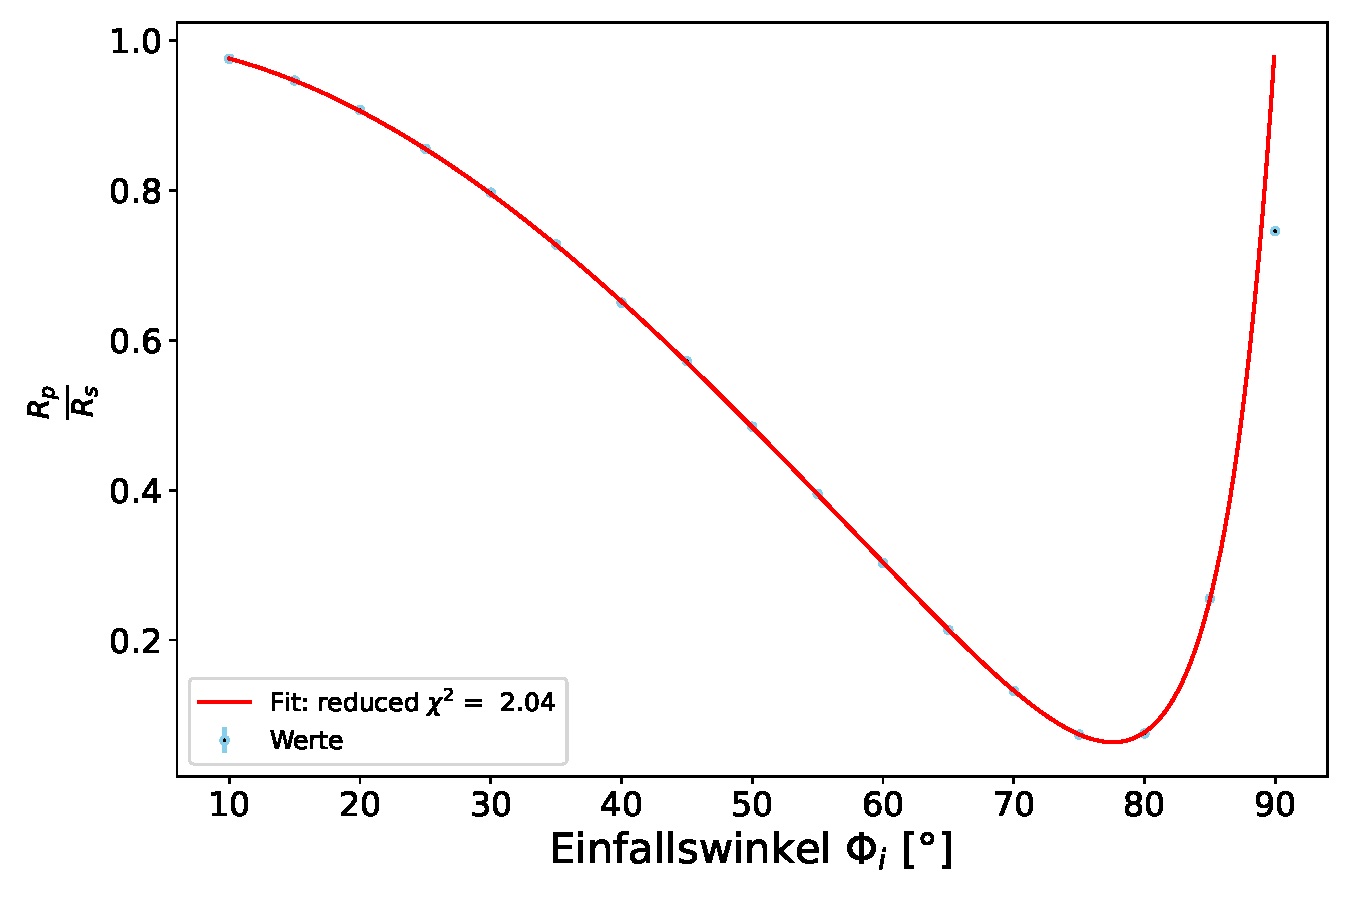
\includegraphics[width= 0.65 \textwidth]{Fits/Rp_Rs_Ge_Fit.pdf} 
	\caption{Rp Rs Ge, Fit} 
 	\label{fig:Rp Rs Ge, Fit} 
\end{figure}
 
\begin{table}[ht] 
	\centering 
	\caption{Rp Rs Ge, Fit Parameter Tabelle} 
	\label{tab: Rp Rs Ge, Fit Parameter Tabelle}
	\begin{tabular}{|l|c|}
		\hline
		Parameter Name	&	Wert \\ \hline
		n	&	 3.982 $\pm$  0.0653\\ \hline
		kappa	&	 2.081 $\pm$  0.0605\\ \hline
	\end{tabular} 
\end{table}
 
\begin{table}[ht] 
	\centering 
	\caption{Rp Rs Ge, Messwerte Tabelle} 
	\label{tab: Rp Rs Ge, Messwerte Tabelle}
	\begin{tabular}{|c|c|}
		\hline
		Einfallswinkel $\Phi_i$ [°] 	&	 $\frac{R_p}{R_s}$\\ \hline
		90.0 $\pm$ 0.2 	&	 0.747 $\pm$ 0.006 \\ \hline
		85.0 $\pm$ 0.2 	&	 0.257 $\pm$ 0.002 \\ \hline
		80.0 $\pm$ 0.2 	&	 0.077 $\pm$ 0.002 \\ \hline
		75.0 $\pm$ 0.2 	&	 0.076 $\pm$ 0.002 \\ \hline
		70.0 $\pm$ 0.2 	&	 0.134 $\pm$ 0.003 \\ \hline
		65.0 $\pm$ 0.2 	&	 0.216 $\pm$ 0.003 \\ \hline
		60.0 $\pm$ 0.2 	&	 0.305 $\pm$ 0.003 \\ \hline
		55.0 $\pm$ 0.2 	&	 0.397 $\pm$ 0.003 \\ \hline
		50.0 $\pm$ 0.2 	&	 0.487 $\pm$ 0.004 \\ \hline
		45.0 $\pm$ 0.2 	&	 0.574 $\pm$ 0.004 \\ \hline
		40.0 $\pm$ 0.2 	&	 0.652 $\pm$ 0.004 \\ \hline
		35.0 $\pm$ 0.2 	&	 0.729 $\pm$ 0.005 \\ \hline
		30.0 $\pm$ 0.2 	&	 0.798 $\pm$ 0.005 \\ \hline
		25.0 $\pm$ 0.2 	&	 0.856 $\pm$ 0.005 \\ \hline
		20.0 $\pm$ 0.2 	&	 0.908 $\pm$ 0.006 \\ \hline
		15.0 $\pm$ 0.2 	&	 0.947 $\pm$ 0.006 \\ \hline
		10.0 $\pm$ 0.2 	&	 0.976 $\pm$ 0.006 \\ \hline
	\end{tabular} 
\end{table}
 
